\chapter{Diseño y arquitectura del sistema}\label{diseno}

En este capítulo se abordará el diseño del sistema. Para ello, a partir del estudio de los métodos y procedimientos disponibles en 
Bro para la gestión de flujos (Apartado \ref{sec.emparejamiento}), se determinarán los módulos y funcionalidades necesarias, 
proponiéndose una arquitectura para el sistema a implementar.

\intro Así, en primer lugar se presentará la arquitectura propuesta y los diferentes módulos y funcionalidades. También se describirán 
las estructuras de datos usadas para la gestión de la información (necesaria).

\section{Arquitectura del sistema}

Para describir la arquitectura del sistema hay que tener en cuenta la arquitectura de Bro. Este monitor de red es un software modular, 
esto es, esta compuesto de diferentes módulos que al ser ejecutados funcionan como un único sistema.

\intro Por lo tanto, la arquitectura del sistema a desarrollar se debe de acoplar a la arquitectura propia de Bro, por lo que el 
sistema debe implementarse como un módulo adicional compatible con Bro. Entre los requisitos del mismo se encuentra que sea ligero y 
eficiente. Por lo tanto, se deberán usar los distintos eventos y capacidades que proporciona Bro para minimizar el impacto en el 
sistema global y optimizar su funcionamiento.

\intro Se prescindirá del uso de los \textit{frameworks} descritos en el capítulo anterior, \ref{sub.framew}, pues su uso no aporta 
nada relevante que no se pueda realizar exclusivamente con los eventos ya disponibles destinados a gestionar el tráfico de la capa de 
transporte. Así, se propone usar este tipo de eventos como núcleo y soporte del módulo y de todas las funcionalidades necesarias. Las 
dos funcionalidades más relevantes del módulo están relacionadas con la evaluación de la similitud entre flujos y la gestión de las 
listas de flujos en diferentes situaciones. Así, se definirá una función que se encargará de evaluar la fórmula del emparejamiento de 
flujos (Apartado \ref{sec.emparejamiento}). Esta función devolverá un número que será el que se compare con el umbral.

\begin{figure}[H]
  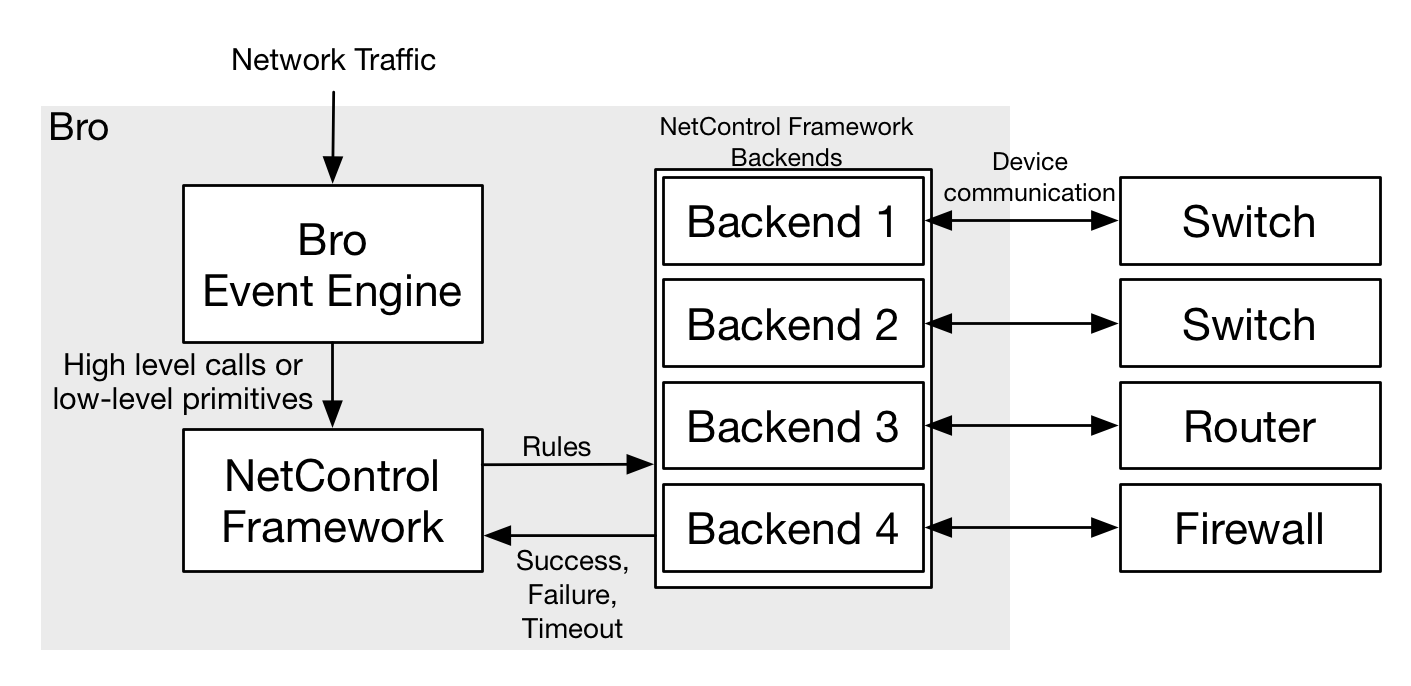
\includegraphics[width=0.9\textwidth]{imagenes/netcarquitectura.png}
  \centering
  \caption{Arquitectura del módulo.}\label{fig.sistema}
\end{figure}

\intro Dependiendo del trato que se les vaya a dar a los flujos detectados se almacenarán en una lista o en otra. Estos pueden estar 
en diferentes estados, siendo estos los que se consideran:

\begin{itemize}
\item Activo. El flujo está activo y almacenado.
\item Emparejado. El flujo ha sido emparejado con otro flujo activo.
\item Finalizado. El flujo ha cumplido su tiempo de vida y es borrado de la memoria.
\end{itemize}

\intro Por lo tanto, como se puede ver en la Figura \ref{fig.flujos}, cuando un flujo es detectado tendrá el estado activo. En función 
de los distintos flujos que se vayan detectando los flujos activos se irán comparando con los nuevos que se detecten, de modo que los 
nuevos que pasarán a estar emparejados. Si no se encuentra un flujo activo que coincida con sus parámetros los nuevos flujos serán 
almacenados como activos. Al último estado, finalizado, se podrá pasar tanto del estado activo, como del emparejado, con la diferencia 
de que de tratarse del primer caso deberá de ser borrado de la lista y se buscará un sustituto entre los emparejados con ese flujo. En 
el segundo caso no se borrará de la lista.

\begin{figure}[H]
  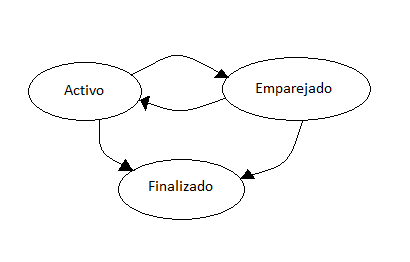
\includegraphics[width=0.9\textwidth]{imagenes/flujos.png}
  \centering
  \caption{Distintos estados de los flujos.}\label{fig.flujos}
\end{figure}

\intro Las entradas de tráfico para su análisis serán trazas en formato \textit{pcap}. Las salidas serán registros, en los cuales se mostrarán los flujos que han sido emparejados. Ampliar!!!

\intro La configuración de Bro, se realiza mediante la línea de comandos, cuando se va a lanzar el programa. Por lo tanto, para el 
módulo que se está describiendo es preciso únicamente activar la opción \textit{-r}, de forma que se le permita leer el archivo que se 
le pasa como parámetro a continuación. En el caso de que se quiera escanear el tráfico de una interfaz, se deberá de activar la opción 
\textit{-i} indicando a continuación el nombre de la interfaz a analizar. Se puede ampliar esta información leyendo la ayuda de Bro con \textit{-h}.

\intro Referenciar a la gestión de flujos

\section{Módulo y funciones}

Las funcionalidades que se espera que tenga este módulo en esencia son dos, la detección y almacenado 
del tráfico y la aplicación de la fórmula para conocer si dos flujos son emparejables, a los distintos flujos que 
se han detectado. De una forma más amplia las funciones del módulo serán las siguientes. 

\begin{itemize}
\item \textit{Función que aplique la fórmula de emparejamiento}. 
\intro A esta función se le pasará dos flujos, de forma que se aplique la fórmula y devuelva un número, el cual 
será el que indique si los flujos son emparejables o no.
\item \textit{Funciones que detecten el tráfico}. 
\intro Esto se hará con los eventos de Bro. Los eventos detectarán el tipo de tráfico que se está analizando 
y aplicarán la función anterior.
\intro Tras el uso de esta fórmula se almacenará o no el flujo que está siendo analizado. Por lo tanto 
será necesario el uso de algún tipo de contenedor para este cometido.
\end{itemize}

\intro Lo que se espera es capturar el tráfico de la capa de transporte. Dicho tráfico se corresponde a los 
protocolos \textit{TCP y UDP}. Por lo tanto será necesario ver que tipo de eventos son los que controlan el tráfico 
de estos dos protocolos. Esto se verá de forma más amplia en la siguiente sección.

\intro Las entradas y salidas son de fácil gestión. Las entradas de tráfico podrán ser mediante archivos o 
analizando directamente el tráfico de la red. Las salidas, por su parte, serán mediante terminal. Esto puede 
suponer cierto inconveniente si se obtienen demasiadas salidas. También se pueden guardar las salidas en un 
fichero mediante el carácter \textit{mayor que} . Con esto se guardará en un fichero en la ruta que se especifique, siendo el 
posterior análisis mucho más cómodo desde, por ejemplo, un editor de texto.

\intro Se debe de tener en cuenta que siempre se podrá extender la funcionalidad del módulo. Pero de momento no 
resulta interesante. La posible extensión correspondería a posibles trabajos futuros.

\intro Para realizar este módulo es necesario conocer como gestiona los flujos Bro y de que forma se mantendrán 
los que son emparejados y los que están activos.

\section{Gestión de flujos}

La gestión de flujos en Bro se realiza completamente con eventos. Por lo cual se tendrán que crear variables 
globales para el almacenamiento de los flujos que sean emparejables y los que estén activos.

\intro El \textit{nacimiento de un flujo} es controlado por un evento. Por lo tanto cuando se detecta un nuevo 
flujo se lanza un evento. Este evento se tendrá que controlar de forma que si se tiene ya un flujo activo con las 
mismas características, se compare y se almacene. Si por el contrario no se tiene ningún flujo con esas 
características se tendrá que almacenar directamente en el contenedor de flujos activos.

\intro La \textit{muerte de un flujo} también es controlada por un evento. Ahora lo importante es si es interesante 
a nivel del análisis seguir almacenando los flujos aunque estos hayan muerto. Si no se quiere tener almacenados 
flujos muertos se tendrá que eliminar de la estructura en la que está almacenado. Si se quiere seguir trabajando 
con ellos habrá que mantenerlos guardados en la estructura. Obviamente si el flujo que va a morir está emparejado 
con otro se borrará solo del contenedor de flujos activos. Manteniéndose en el contenedor de flujos emparejados. De 
lo contrario se perderá información. Todo esto habrá que decidirlo en el evento que gestiona la muerte del flujo.

\intro Estos dos comportamientos de los flujos están controlados por eventos genéricos. Con un único evento se 
detecta que el flujo ha nacido y con otro evento si ha muerto, independientemente del tipo de protocolo al que 
pertenezca. No pasará esto con los distintos estados de los flujos que serán detectados. Pues no es lo mismo 
detectar un ACK de un flujo TCP que una respuesta de un flujo UDP. Serán tratados en eventos distintos y tendrán que ser gestionados con eventos distintos, cada uno destinado a un protocolo distinto. 

\intro A continuación se verán las estructuras de datos necesarias para llevar a cabo el desarrollo del módulo.

\section{Estructuras de datos}

Las principales estructuras de datos que se necesitan para el desarrollo de este trabajo serán dos 
tablas, \textit{table} \cite{brotable}, de vectores para el almacenamiento de los flujos activos y los emparejados. 
Los vectores son iguales que en cualquier otro lenguaje de programación, mientras que las tablas son parecidas a los \textit{maps} de \textit{C++}. Aunque esto se podrá ver con mejor detalle en el apartado de implementación.

\intro Dichas estructuras de almacenamiento, deberán de ser capaces de estar ordenadas por las IP's y los puertos. 
Lo cual se obtiene juntando las tablas con los vectores para así conseguir una especie de matriz bidimensional, 
la cual está indexada. Por lo tanto se consigue que el acceso a los datos sea mucho más rápido. Incluso se podría 
prescindir de bucles, los cuales pueden acabar siendo un problema en cuanto a rendimiento si se llega a almacenar 
muchos flujos.

\intro Bro proporciona cierto tipos de datos muy interesantes, los cuales además, incluyen mucha más información. 
Algunos de estos tipos de datos son. 

\begin{itemize}

\item \textit{connection}. 

\intro Este tipo de dato es el flujo en si. Por lo tanto será de vital importancia comprenderlo para poder trabajar 
como se desea.

\intro Dentro del tipo de dato \textit{connection} existe un registro llamado \textit{id}, el cual esta 
compuesto por el tipo de dato \textit{conn\_id} \cite{broconnid}. Este dato sirve para identificar los flujos 
mediante una tupla formada por 4 datos. Estos datos son los que se precisan para indexar la matriz bidimensional, 
siendo pues las IP's y los puertos.

  \begin{itemize}

  \item \textit{addr}. Este tipo de dato representa una IP. Reconoce tanto IPv4 como IPv6. Este tipo de dato puede 
  ser comparado e incluso ordenado mediante operadores. \cite{broaddr}

  \item \textit{port}. Este tipo es el usado para los puertos. Además del número de puerto también indica el 
  protocolo de la capa de transporte que usa. Soporta la comparación y ordenación, pero no por el número, sino por 
  el tipo de protocolo. \cite{broport}
  \end{itemize}
  
\intro Para obtener más información sobre el tipo de dato \textit{connection} lea \cite{connectiontype}.

\item \textit{time}. 

\intro Este tipo de dato también es interesante. Aunque en otros lenguajes se puede obtener, 
en Bro es un tipo de dato por si mismo. Por lo tanto se podrá operar sobre él desde el principio, siendo una gran 
ventaja a la hora de calcular el tiempo de inicio de los flujos. Para leer más \cite{timetype}. 

\intro Es importante entender que para realizar el cálculo para el emparejamiento de flujos, se necesita el 
\textit{timestamp} del primer paquete de cada flujo, pues será sobre este tiempo sobre el que se apoye el 
cálculo del emparejamiento.

\end{itemize}

\intro Estos dos tipos de datos a parte de ser los más interesantes para el cálculo del emparejamiento, también 
serán los más utilizados junto a los contenedores para los flujos. Existen más tipos de datos e incluso los hay que 
extienden la información disponible sobre los flujos. Para leer más sobre esto \cite{conntype}.
